\documentclass[handout,10pt]{beamer}
\usepackage{SexySlides,fancyvrb,outlines,pbox}
\usepackage[round]{natbib}
\usepackage{hyperref} % link references

\definecolor{UniBlue}{RGB}{83,121,170}
\setbeamercolor{title}{fg=UniBlue}
\setbeamercolor{frametitle}{fg=UniBlue}
\newcommand{\coluit}{\color{UniBlue}\it}
\newcommand{\colubf}{\color{UniBlue}\bf}

\DeclareMathOperator*{\diag}{diag}
\DeclareMathOperator*{\Tr}{Tr}
\DeclareMathOperator*{\argmin}{argmin}

     \setbeamertemplate{footline}
        {
      \leavevmode%
      \hbox{%
      \begin{beamercolorbox}[wd=.333333\paperwidth,ht=2.25ex,dp=1ex,center]{author in head/foot}%
        \usebeamerfont{author in head/foot}\insertshortauthor~~
        %(\insertshortinstitute)
      \end{beamercolorbox}%
      \begin{beamercolorbox}[wd=.333333\paperwidth,ht=2.25ex,dp=1ex,center]{title in head/foot}%
        \usebeamerfont{title in head/foot}\insertshorttitle
      \end{beamercolorbox}%
      \begin{beamercolorbox}[wd=.333333\paperwidth,ht=2.25ex,dp=1ex,right]{date in head/foot}%
        \usebeamerfont{date in head/foot}\insertshortdate{}\hspace*{2em}

    %#turning the next line into a comment, erases the frame numbers
        %\insertframenumber{} / \inserttotalframenumber\hspace*{2ex} 

      \end{beamercolorbox}}}%

%\def\logo{%
%{\includegraphics[height=1cm]{goldy1.png}}
%}
%%
%\setbeamertemplate{footline}
%{%
%	\hspace*{.05cm}\logo
%  \begin{beamercolorbox}[sep=1em,wd=10cm,rightskip=0.5cm]
%  {footlinecolor,author in head/foot}
%%    \usebeamercolor{UniBlue}
%    \vspace{0.1cm}
%    \insertshortdate \hfill \insertshorttitle
%    \newline
%    \insertshortauthor   - \insertshortinstitute
%    \hfill
%    \hfill \insertframenumber/\inserttotalframenumber
%  \end{beamercolorbox}
%  \vspace*{0.05cm}
%}

%% smart verbatim
\fvset{framesep=1cm,fontfamily=courier,fontsize=\scriptsize,framerule=.3mm,numbersep=1mm,commandchars=\\\{\}}

\title[Depth PCA]
{\Large  
Robust estimation of \\principal components from \\depth-based multivariate rank covariance matrix}

\author[Subho Majumdar]{Subho Majumdar\\ Snigdhansu Chatterjee}
\institute[]{University of Minnesota, School of Statistics\\
\vspace{.5cm}

\includegraphics[height=.5cm]{UMNlogo}}

\date {}

\date [August 9, 2015]

%%%%%%%List Outline in the beginning of each section.
%\AtBeginSection[] {
%   \begin{frame}
%       \frametitle{Outline}
%       \tableofcontents[currentsection]
%   \end{frame}
%}

%-------------------------------------------------------------------
\begin{document}

%\begin{frame}
\frame{ \titlepage}
%\end{frame}

\frame{\frametitle{Table of contents}\tableofcontents}

%---------------------------------------------------

\begin{frame}
\frametitle{Summary}
\begin{itemize}
\item Introduction: what is data depth?
\vspace{.5cm}
\item Multivariate ranks based on data depth
\vspace{.5cm}
\item The Depth Covariance Matrix (DCM): overview of results
\vspace{.5cm}
\item Performance: simulations and real data analysis
\end{itemize}
\end{frame}

\begin{frame}
\frametitle{What is depth?}
\textbf{Example}: 500 points from $\mathcal{N}_2 ((0,0)^T, \diag (2,1))$
\begin{figure}\begin{center}
   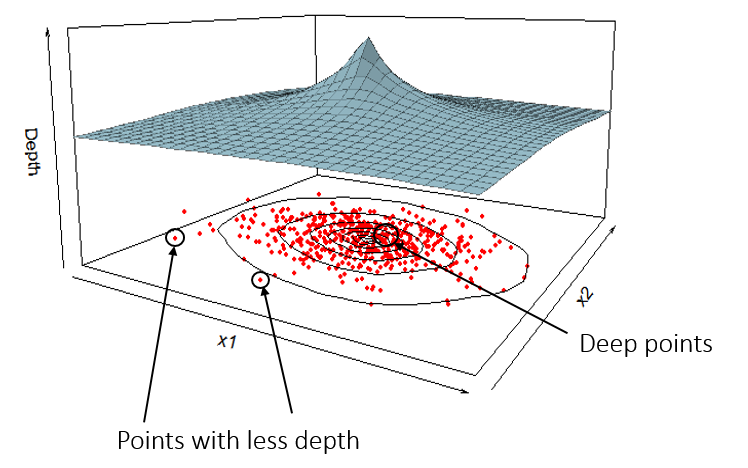
\includegraphics[height=6cm]{depthplot}
   \label{fig:fig1}
\end{center}\end{figure}
\colbbf{A scalar measure of how much inside a point is with respect to a data cloud}
\end{frame}

\begin{frame}
\frametitle{Formal definition}
For any multivariate distribution $F = F_\bfX$, the depth of a point $\bfx \in \mathbb{R}^p$, say $D(\bfx, F_\bfX)$ is any real-valued function that provides a `center outward ordering' of $\bfx$ with respect to $F$ \citep{zuo00}.

\vspace{.5cm}
\begin{block}{Desirable properties \citep{liu90}}
(P1) {\colbit Affine invariance}: $D(A\bfx + \bfb, F_{A\bfX+\bfb}) = D(\bfx, F_\bfX)$
\vspace{.2cm}

(P2) {\colbit Maximality at center}: $D(\bftheta, F_\bfX) = \sup_{\bfx\in \mathbb{R}^p} D(\bfx, F_\bfX)$ for $F_\bfX$ with center of symmetry $\bftheta$, the \textit{deepest point} of $F_\bfX$.
\vspace{.2cm}

(P3) {\colbit Monotonicity w.r.t. deepest point}: $D(\bfx; F_\bfX) \leq D(\bftheta + a(\bfx - \bftheta), F_\bfX)$
\vspace{.5cm}

(P4) {\colbit Vanishing at infinity}: $D(\bfx; F_\bfX) \rightarrow \bf0$ as $\|\bfx\| \rightarrow \infty $.
\end{block}
\end{frame}

\begin{frame}
\frametitle{Examples}
\begin{itemize}
\item \textbf{Halfspace depth} (HD) \citep{tukey75} is the minimum probability of all halfspaces containing a point.
$$ HD(\bfx, F)  = \inf_{\bfu \in \mathbb{R}^p; \bfu \neq \bf0} P(\bfu^T \bfX \geq \bfu^T \bfx) $$

\item \textbf{Projection depth} (PD) \citep{zuo03} is based on an outlyingness function:
$$ O(\bfx, F) = \sup_{\| \bfu \| = 1} \frac{| \bfu^T\bfx - m(\bfu^T\bfX)|}{s(\bfu^T\bfX)}; \quad PD(\bfx, F) = \frac{1}{1+O(\bfx, F)} $$
\end{itemize}
\end{frame}

\begin{frame}
\frametitle{Utility of data depth}
{\colbbf Robustness}

\begin{itemize}
\item \textbf{Classification}
\vspace{.2cm}

\item Depth-weighted means and covariance matrices
\vspace{.2cm}

\item What we're going to do:\\Define multivariate rank vectors based on data depth, do PCA on them
\end{itemize}
\end{frame}

\begin{frame}
\frametitle{Spatial signs \citep{locantore99}}
$$ \bfS(\bfx) = \begin{cases} \bfx\| \bfx \|^{-1} \quad \mbox{if }\bfx \neq \bf0\\
\bf0 \quad \mbox{if }\bfx = \bf0 \end{cases} $$

\begin{itemize}
\item Say $\bfx$ follows an elliptic distribution with mean $\bfmu$, covariance matrix $\Sigma$.
\item Sign covariance matrix (SCM): $\Sigma_S(\bfX) = E\bfS (\bfX - \bfmu)\bfS (\bfX - \bfmu)^T$
\item SCM has same eigenvectors as $\Sigma$. PCA using SCM is robust, but not efficient.
\end{itemize}

\begin{figure}\begin{center}
   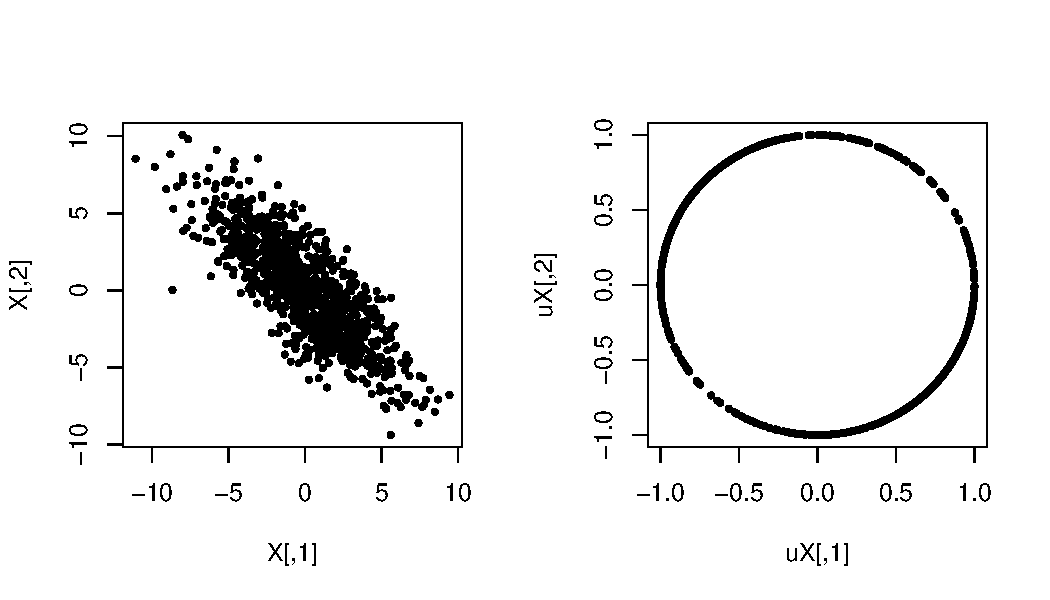
\includegraphics[height=5cm]{signs}
   \label{fig:fig2}
\end{center}\end{figure}
\end{frame}

\begin{frame}
\frametitle{Spatial ranks}

\begin{itemize}
\item Fix a depth function $D(\bfx, F) = D_\bfX(\bfx)$. Define $ \tilde D_\bfX(\bfx) = \sup_{\bfx\in \mathbb{R}^p} D_\bfX(\bfx) - D_\bfX(\bfx) $

\item Transform the original observation: $\tilde \bfx = \tilde D_\bfX(\bfx) \bfS(\bfx - \bfmu)$. This is the {\colbit Spatial Rank} of $\bfx$.

\item Depth Covariance Matrix (DCM) = $Cov(\tilde \bfX)$. Has more information than spatial signs, so more efficient.
\end{itemize}

\begin{figure}\begin{center}
   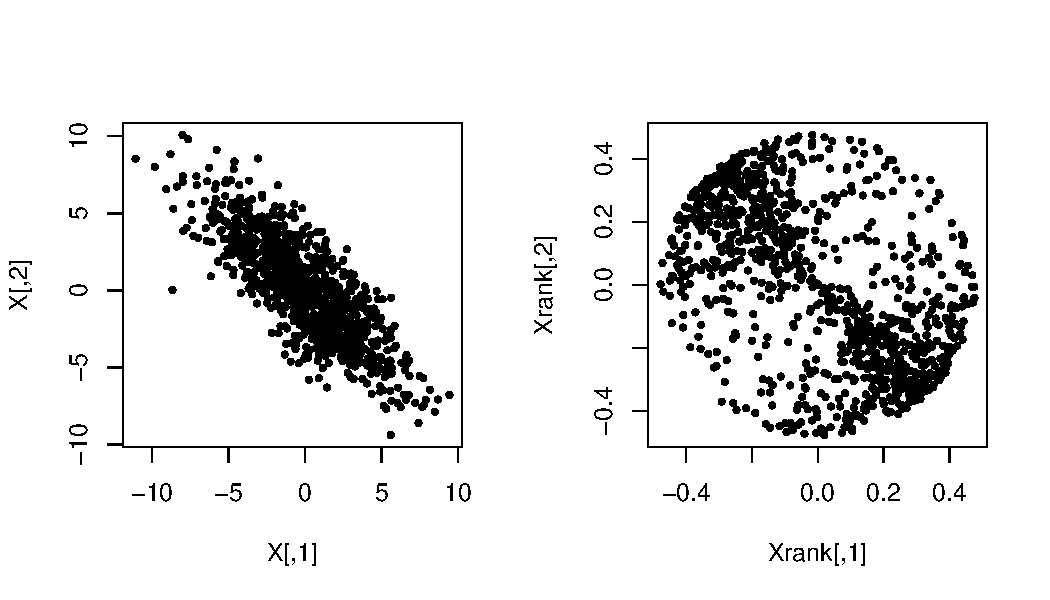
\includegraphics[height=5cm]{ranks}
   \label{fig:fig3}
\end{center}\end{figure}
\end{frame}

\begin{frame}
\frametitle{Form of DCM}
\begin{theorem}[1]
Let the random variable $\bfX \in \mathbb{R}^p$ follow an elliptical distribution with center $\bfmu$ and covariance matrix $\Sigma = \Gamma\Lambda\Gamma^T$, its spectral decomposition. Then, given a depth function $D_\bfX(.)$ the covariance matrix of the transformed random variable $\tilde\bfX$ is
\begin{equation}
Cov(\tilde \bfX) = \Gamma \Lambda_{D,S} \Gamma^T,\quad\mbox{with}\quad \Lambda_{D,S} = E \left[ (\tilde D_\bfZ(\bfz))^2 \frac{\Lambda^{1/2} \bfz \bfz^T \Lambda^{1/2}}{\bfz^T \Lambda \bfz} \right]
\end{equation}

where $\bfz = (z_1,...,z_p)^T \sim N({\bf 0}, I_p)$ and $\Lambda_{D,S}$ a diagonal matrix with diagonal entries
$$ \lambda_{D,S,i} = E_\bfZ \left[ \frac{(\tilde D_\bfZ(\bfz))^2 \lambda_i z_i^2}{\sum_{j=1}^p \lambda_j z_j^2} \right] $$
\end{theorem}

\vspace{.5cm}
{\colb \textbf{TL; DR:} Population eigenvectors are invariant under the spatial rank transformation.}
\end{frame}

\begin{frame}
\frametitle{Other results}
\begin{itemize}
\item Asymptotic distribution of sample DCM, form of its asymptotic variance
\vspace{.2cm}

\item Asymptotic joint distribution of eigenvectors and eigenvalues of sample DCM
\vspace{.2cm}

\item Form and shape of influence function: a measure of robustness
\vspace{.2cm}

\item Asymptotic efficiency relative to sample covariance matrix
\end{itemize}
\end{frame}

\begin{frame}
\frametitle{Simulation}
\begin{itemize}
\item 6 elliptical distributions: $p$-variate normal and $t$- distributions with df = 5, 6, 10, 15, 25.
\vspace{.2cm}

\item All distributions centered at ${\bf 0}_p$, and have covariance matrix $\Sigma = \diag(p,p-1,...1)$. 
\vspace{.2cm}

\item 3 choices of $p$: 2, 3 and 4.
\vspace{.2cm}

\item 10000 samples each for sample sizes $n = 20, 50, 100, 300, 500$
\vspace{.2cm}

\item For estimates $\hat\bfgamma_1$ of the first eigenvector $\hat\bfgamma_1$, prediction error is measured by the average smallest angle between the two lines, i.e. \textbf{Mean Squared Prediction Angle}:
$$ MSPA(\hat \bfgamma_1) = \frac{1}{10000} \sum_{m=1}^{10000} \left( \cos^{-1} \left|\bfgamma_1^T \hat\bfgamma^{(m)}_1 \right| \right)^2 $$

Finite sample efficiency of some eigenvector estimate $\hat\bfgamma^E_1$ relative to that obtained from the sample covariance matrix, say $\hat\bfgamma^{Cov}_1$ is:
$$ FSE(\hat\bfgamma^E_1, \hat\bfgamma^{Cov}_1) = \frac{MSPA(\hat\bfgamma^{Cov}_1)}{MSPA(\hat\bfgamma^E_1)} $$
\end{itemize}
\end{frame}

\begin{frame}
\frametitle{Table of FSE for $p=2$}

(HSD = Halfspace depth, MhD = Mahalanobis depth, PD = Projection depth)
\begin{table}
\begin{footnotesize}
   \begin{tabular}{c|cccc}
    \hline
    $F$ = Bivariate $t_5$      & SCM  & HSD-CM & MhD-CM & PD-CM \\ \hline
    $n$=20                        & 0.80 & 0.95   & 0.95   & 0.89  \\
    $n$=50                        & 0.86 & 1.25   & 1.10   & 1.21  \\
    $n$=100                       & 1.02 & 1.58   & 1.20   & 1.54  \\
    $n$=300                       & 1.24 & 1.81   & 1.36   & 1.82  \\
    $n$=500                       & 1.25 & 1.80   & 1.33   & 1.84  \\ \hline
    $F$ = Bivariate $t_6$      & SCM  & HSD-CM & MhD-CM & PD-CM \\ \hline
    $n$=20                        & 0.77 & 0.92   & 0.92   & 0.86  \\
    $n$=50                        & 0.76 & 1.11   & 1.00   & 1.08  \\
    $n$=100                       & 0.78 & 1.27   & 1.06   & 1.33  \\
    $n$=300                       & 0.88 & 1.29   & 1.09   & 1.35  \\
    $n$=500                       & 0.93 & 1.37   & 1.13   & 1.40  \\ \hline
    $F$ = Bivariate $t_{10}$ & SCM  & HSD-CM & MhD-CM & PD-CM \\ \hline
    $n$=20                        & 0.70 & 0.83   & 0.84   & 0.77  \\
    $n$=50                        & 0.58 & 0.90   & 0.84   & 0.86  \\
    $n$=100                       & 0.57 & 0.92   & 0.87   & 0.97  \\
    $n$=300                       & 0.62 & 0.93   & 0.85   & 0.99  \\
    $n$=500                       & 0.62 & 0.93   & 0.86   & 1.00  \\ \hline
    \end{tabular}
\end{footnotesize}
\label{table:FSEtable1}
\end{table}
\end{frame}

\begin{frame}
\frametitle{Table of FSE for $p=2$}
(HSD = Halfspace depth, MhD = Mahalanobis depth, PD = Projection depth)
\begin{table}
\begin{footnotesize}
   \begin{tabular}{c|cccc}
    \hline
    $F$ = Bivariate $t_{15}$ & SCM  & HSD-CM & MhD-CM & PD-CM \\ \hline
    $n$=20                        & 0.63 & 0.76   & 0.78   & 0.72  \\
    $n$=50                        & 0.52 & 0.79   & 0.75   & 0.80  \\
    $n$=100                       & 0.51 & 0.83   & 0.77   & 0.88  \\
    $n$=300                       & 0.55 & 0.84   & 0.79   & 0.91  \\
    $n$=500                       & 0.56 & 0.85   & 0.80   & 0.93  \\ \hline
    $F$ = Bivariate $t_{25}$ & SCM  & HSD-CM & MhD-CM & PD-CM \\ \hline
    $n$=20                        & 0.63 & 0.77   & 0.79   & 0.74  \\
    $n$=50                        & 0.49 & 0.73   & 0.71   & 0.76  \\
    $n$=100                       & 0.45 & 0.73   & 0.69   & 0.81  \\
    $n$=300                       & 0.51 & 0.78   & 0.75   & 0.87  \\
    $n$=500                       & 0.53 & 0.79   & 0.75   & 0.87  \\ \hline
    $F$ = BVN                     & SCM  & HSD-CM & MhD-CM & PD-CM \\ \hline
    $n$=20                        & 0.56 & 0.69   & 0.71   & 0.67  \\
    $n$=50                        & 0.42 & 0.66   & 0.66   & 0.70  \\
    $n$=100                       & 0.42 & 0.69   & 0.66   & 0.77  \\
    $n$=300                       & 0.47 & 0.71   & 0.69   & 0.82  \\
    $n$=500                       & 0.48 & 0.73   & 0.71   & 0.83  \\ \hline
    \end{tabular}
\end{footnotesize}
\label{table:FSEtable2}
\end{table}
\end{frame}

\begin{frame}
\frametitle{Data analysis: Bus data}
\begin{itemize}
\item Features extracted from images of 213 buses: 18 variables
\vspace{.2cm}

\item Methods compared:\\
\vspace{.2cm}
Classical PCA (CPCA)\\
SCM PCA (SPCA)\\
ROBPCA \citep{hubert05}\\
PCA based on MCD (MPCA)\\
PCA based on projection-DCM (DPCA)
\vspace{.2cm}
\end{itemize}
\end{frame}

\begin{frame}
\frametitle{Score distance (SD) and orthogonal distance (OD)}
$$ SD_i = \sqrt{ \sum_{j=1}^k \frac{s^2_{ij}}{\lambda_j}}; \quad OD_i = \| \bfx_i - P\bfs_i^T \| $$

\begin{footnotesize}
where $S_{n\times k} = (\bfs_1, \ldots ,\bfs_n)^T$ is the scoring matrix, $P_{p\times k}$ loading matrix, $\lambda_1,\ldots ,\lambda_k$ are eigenvalues obtained from the PCA, and $\bfx_1,\ldots,\bfx_n$ are the observation vectors.
\end{footnotesize}

\begin{figure}[h]
	\centering
		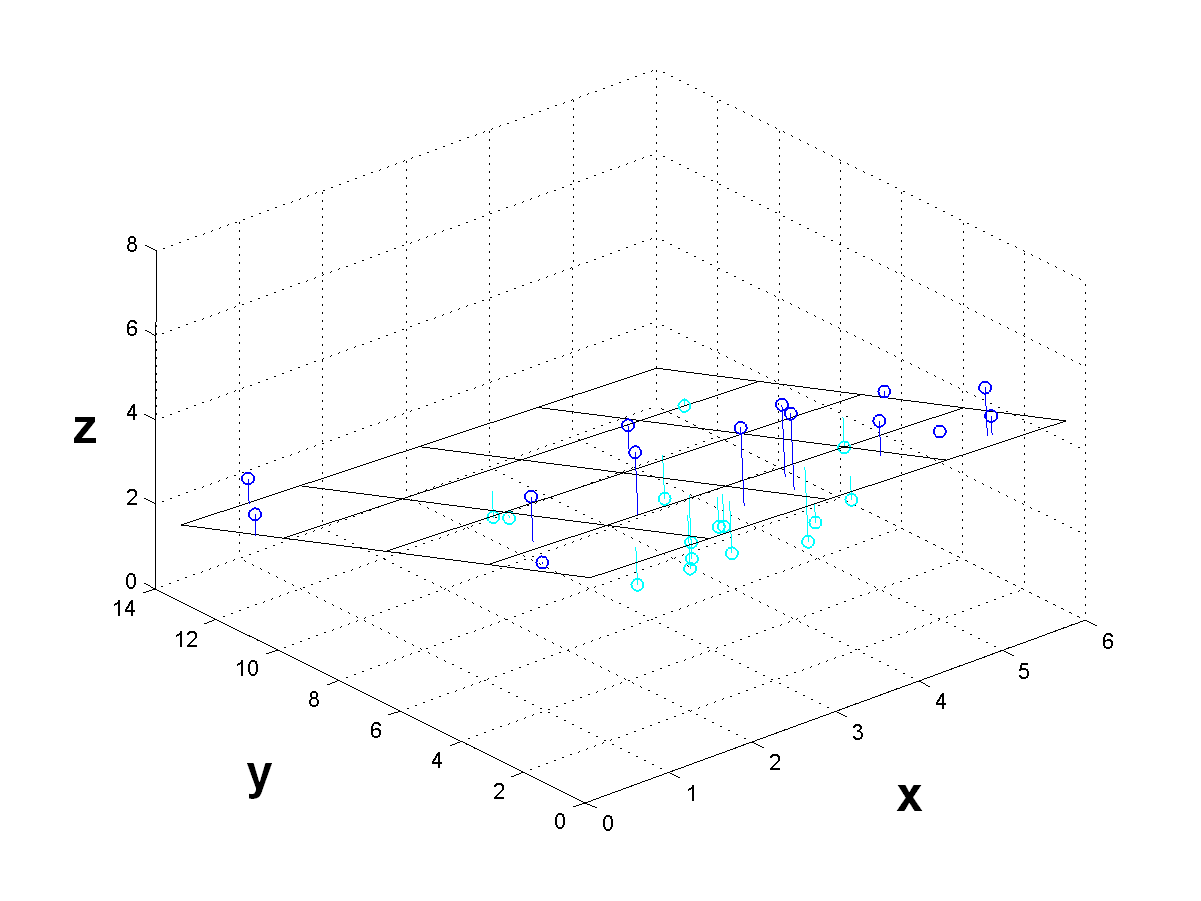
\includegraphics[height=5.5cm]{ScoreOrtho}
	\label{fig:ScoreOrthoPlot}
\end{figure}
\end{frame}

\begin{frame}
\frametitle{Bus data: comparison tables}

\begin{footnotesize}
\begin{table}[t]
\centering
    \begin{tabular}{c|ccccc}
    \hline
    Quantile & \multicolumn{5}{c}{Method of PCA}         \\ \cline{2-6}
    ~                   & CPCA     & SPCA & ROBPCA & MPCA & DPCA \\\hline 
    10\%      & 1.9       & {\colb 1.2}       & {\colm 1.2}    & {\colr 1.0}       & {\colubf 1.2}       \\
    20\%      & 2.3       & {\colb 1.6}       & {\colm 1.6}    & {\colr 1.3}       & {\colubf 1.6}       \\
    30\%      & 2.8       & {\colb 1.8}       & {\colm 1.8}    & {\colr 1.7}       & {\colubf 1.9}       \\
    40\%      & 3.2       & {\colb 2.2}       & {\colm 2.1}    & {\colr 2.1}       & {\colubf 2.3}       \\
    50\%      & 3.7       & {\colb 2.6}       & {\colm 2.5}    & {\colr 3.1}       & {\colubf 2.6}       \\
    60\%      & 4.4       & {\colb 3.1}       & {\colm 3.0}    & 5.9       & {\colubf 3.2}       \\
    70\%      & 5.4       & {\colb 3.8}       & {\colm 3.9}    & 25.1      & {\colubf 3.9}       \\
    80\%      & 6.5       & {\colb 5.2}       & {\colm 4.8}    & 86.1      & {\colubf 4.8}       \\
    90\%      & 8.2       & 9.0       & 10.9   & 298.2     & {\colubf 6.9}      \\
    Max       & 24        & 1037      & 1055   & 1037      & 980      \\\hline
    \end{tabular}
    \label{table:bus_table2}
\end{table}
\end{footnotesize}

\begin{itemize}
\item Table lists quantiles of the squared orthogonal distance for a sample point from the hyperplane formed by top 3 PCs,
\vspace{.2cm}
\item For DPCA, more than 90\% of points have a smaller orthogonal distance than CPCA
\end{itemize}
\end{frame}

\begin{frame}
\frametitle{Data analysis: Octane data}
\begin{itemize}
\item 226 variables and 39 observations. Each observation is a gasoline sample with a certain octane number, and have their NIR absorbance spectra measured in 2 nm intervals between 1100 - 1550 nm.
\vspace{.2cm}
\item 6 outliers: compounds 25, 26 and 36-39, which contain alcohol.
\end{itemize}

\begin{figure}[h]
	\centering
		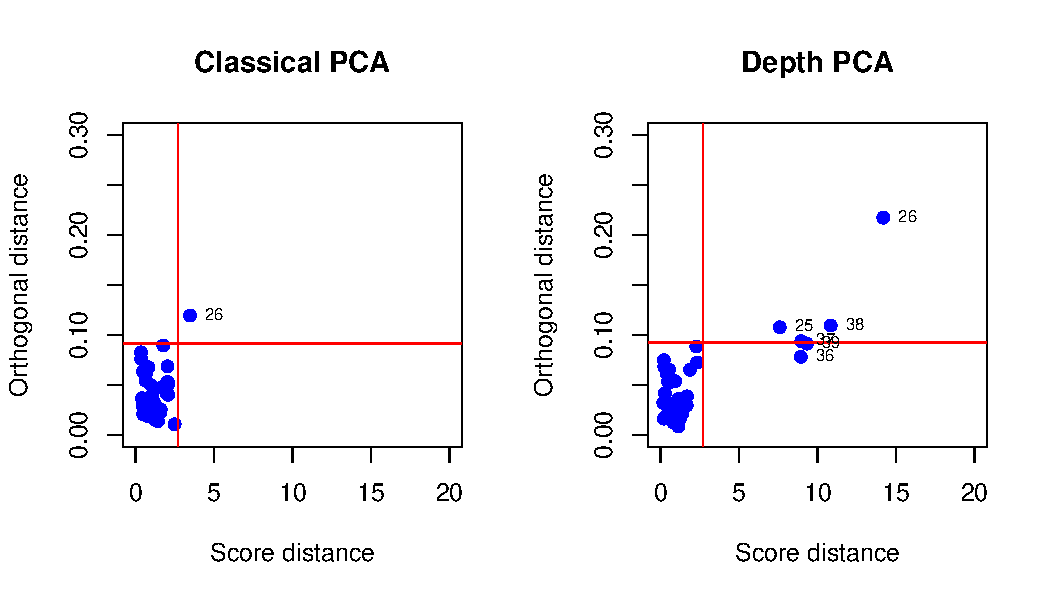
\includegraphics[height=6cm]{octane_distanceplot.pdf}
	\label{fig:distplot}
\end{figure}
\end{frame}

\begin{frame}
\frametitle{Extensions: Robust kernel PCA}

\begin{footnotesize}
\begin{itemize}
\item 20 points from each person. Noise added to one image from each person.
\item Columns due to kernel CPCA, SPCA and DPCA, respectively. Rows due to top 2, 4, 6, 8 or 10 PCs considered.
\end{itemize}
\end{footnotesize}

\begin{figure}[h]
	\centering
		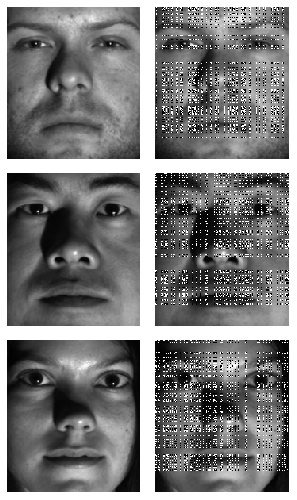
\includegraphics[width=2cm]{yale1.png}
		\hspace{.2cm}
		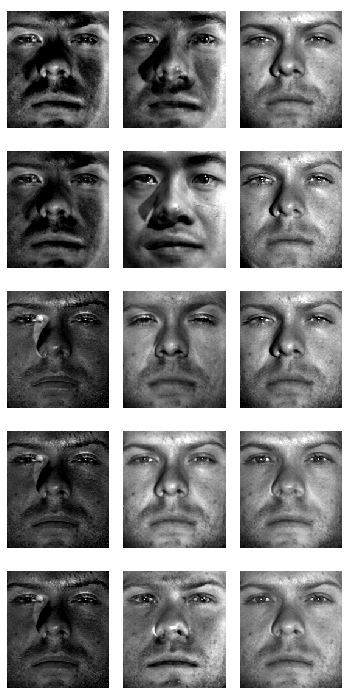
\includegraphics[width=3cm]{yaleB01recon.png}
		\hspace{.2cm}
		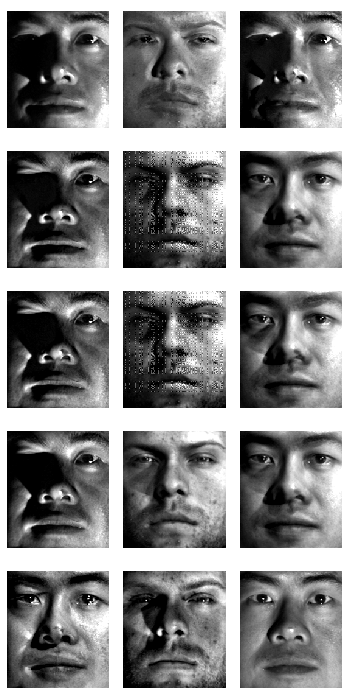
\includegraphics[width=3cm]{yaleB02recon.png}
		\hspace{.2cm}
		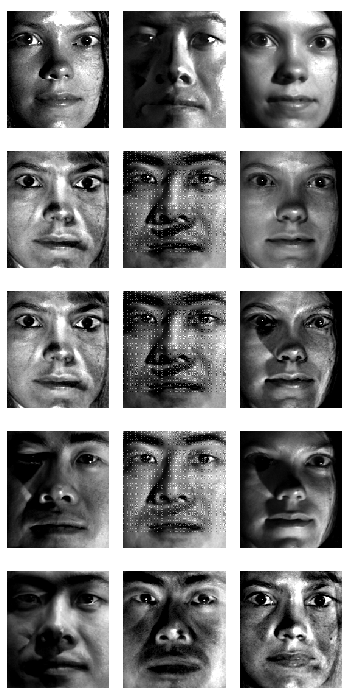
\includegraphics[width=3cm]{yaleB28recon.png}
	\label{fig:kdpca}
\end{figure}
\end{frame}

\begin{frame}
\frametitle{Extensions: future work}
\begin{itemize}
\item Explore properties of a depth-weighted M-estimator of scale matrix:
$$ \Sigma_{Dw} = E \left[ \frac{(\tilde D_\bfX(\bfx))^2 (\bfx - \bfmu) (\bfx - \bfmu)^T}{(\bfx - \bfmu)^T \Sigma_{Dw}^{-1} (\bfx - \bfmu)} \right] $$
\vspace{.5cm}

\item Leverage the idea of depth based ranks: robust non-parametric testing

\item Extending to high-dimensional and functional data
\end{itemize}
\end{frame}

\begin{frame}
\frametitle{Acknowledgements}
\begin{itemize}
\item NSF grants \# IIS-1029711, \# SES-0851705;
\vspace{.2cm}
\item NASA grant \#-1502546;
\vspace{.2cm}
\item The Institute on the Environment (IonE), and College of Liberal Arts (CLA) - University of Minnesota;
\vspace{.2cm}
\item Abhirup Mallik;
\vspace{.2cm}
\item My team in Santander Consumer USA;
\end{itemize}
\end{frame}

\begin{frame}
\frametitle{References}
\bibliographystyle{plainnat}
\bibliography{scatterbib}
\end{frame}


\begin{frame}
\centering\huge
\textcolor{UniBlue}{\textbf{THANK YOU!}}
\end{frame}

\end{document}